\documentclass{beamer}
\usepackage[utf8]{inputenc}
\usepackage[T1]{fontenc}
\usepackage{amsmath, amsthm}
\usepackage{python}
\usepackage{listings}
\usepackage{float}
\usepackage{graphicx}
\usepackage{subcaption}
% \usepackage{amssymb}
% \usepackage{algorithm}
% \usepackage{nccmath}

% \newtheorem{theorem}{Theorem}[section]
% \newtheorem{lemma}[theorem]{Lemma}
% \newtheorem{proposition}[theorem]{Proposition}
% \newtheorem{corollary}[theorem]{Corollary}
% % \theoremstyle{definition} %Makes def,ex and remark without italics
% \newtheorem{definition}[theorem]{Definition}
% \newtheorem{example}[theorem]{Example}
% \newtheorem{remark}[theorem]{Remark}


\newcommand{\quoteswe}[1]{”#1”}
\newcommand{\quoteeng}[1]{“#1”}

\newcommand{\norm}[1]{\left\lVert#1\right\rVert}
\newcommand{\abs}[1]{\left| #1 \right|}
\newcommand{\inner}[2]{\left< #1 , #2 \right>}
\renewcommand{\Re}{\operatorname{Re}}
\renewcommand{\Im}{\operatorname{Im}}
\renewcommand{\phi}{\varphi}
\renewcommand{\Phi}{\varPhi}
\newcommand{\sgn}[1]{\operatorname{sgn} (#1)}
\newcommand{\csgn}[1]{\operatorname{csgn} (#1)}
\newcommand{\argmin}[1]{\underset{#1}{\arg\min}}
\newcommand{\Arg}{\operatorname{Arg}}
\renewcommand{\exp}[1]{\operatorname{e}^{#1}}
\newcommand{\expalt}{\operatorname{exp}}
\renewcommand{\i}{\mathrm{i}}
\newcommand{\id}{\mathrm{I}}
\newcommand{\T}{\mathrm{T}}
\newcommand{\coi}[2]{\left[#1, #2\right]}

\makeatletter
\newenvironment<>{proofs}[1][\proofname]{%
    \par
    \def\insertproofname{#1\@addpunct{.}}%
    \usebeamertemplate{proof begin}#2}
  {\usebeamertemplate{proof end}}
\newenvironment<>{proofc}{%
  \setbeamertemplate{proof begin}{\begin{block}{}}
    \par
    \usebeamertemplate{proof begin}}
  {\usebeamertemplate{proof end}}
\newenvironment<>{proofe}{%
    \par
    \pushQED{\qed}
    \setbeamertemplate{proof begin}{\begin{block}{}}
    \usebeamertemplate{proof begin}}
  {\popQED\usebeamertemplate{proof end}}
\makeatother

\usetheme{Boadilla}
\title{Relaxation Runge-Kutta Methods and Entropy Stability}
% \subtitle{}
\author{Thomas Renström}
\institute{Lund University}
\date{\today}


\begin{document}

\begin{frame}
    \titlepage
\end{frame}

\section{Introduction}

\begin{frame}{Introduction}
    Why do we want entropy stabile methods?
\end{frame}

\section{Preliminaries}
\begin{frame}{ODE}
    \vspace*{-2cm}
    % We consider a time-dependent ODE of the form
    \begin{align*}
        \frac{\text{d}}{\text{d}t} u(t) &= f(t, u(t)), \quad t \in (0, T)\\
        u(0) &= u^0
    \end{align*}
    \(u \in \mathcal{H}\) real Hilbert space with the inner product \(\inner{\cdot}{\cdot}\), inducing the norm \(\norm{\cdot}\).
\end{frame}

\begin{frame}{Entropy}
    % We denote by
    \[ \eta: \mathcal{H} \rightarrow \mathbb{R}\]
    smooth convex function in time.
    % We call this entropy, while in other application it might instead represent some form of energy or momentum.

    \vspace*{10mm}
    E.g. entropy, energy or momentum.

\end{frame}

\begin{frame}{Entropy 2}
    % The change in entropy over time is given by
    \[\frac{\text{d}}{\text{d}t} \eta (u(t)) = \inner{\eta'(u(t))}{f(t, u(t))}.\]
    % A entropy dissipative system will satisfy

    \vspace*{5mm}
    Entropy dissipative:
    \[\inner{\eta'(u(t))}{f(t, u(t))} \leq 0, \quad \forall u \in \mathcal{H}, t \in [0, T],\]
    % and a entropy conservative system will satisfy
    Entropy conservative:
    \[\inner{\eta'(u(t))}{f(t, u(t))} = 0, \quad \forall u \in \mathcal{H}, t \in [0, T].\]
\end{frame}

\begin{frame}{Classic Runge-Kutta}
    % A general Runge-Kutta method with \(s\) stages is represented with the Butcher tableau
    Butcher tableau
    \[\begin{array}{c|c}
        c & A\\
        \hline
        ~ & b^{\T}
    \end{array},
    \qquad A \in \mathbb{R}^{s \times s} \text{ and } b, c \in \mathbb{R}^s
    \]
    Scheme
    \begin{align*}
        y_i &= u^{n} + \Delta t\sum_{j=1}^{s} a_{i,j} f(t_n + c_j \Delta t, y_j), \quad i = 1,\ldots,s\\
        u^{n+1} &= u^{n} + \Delta t \sum_{i=1}^{s} b_i f(t_n + c_i \Delta t, y_i).
    \end{align*}

    \vspace*{5mm}
    We introduce the notation
    \[f_i = f(t_n + c_i \Delta t, y_i), \qquad f_0 = f(t_n, u^n).\]
\end{frame}

\section{Relaxation Runge-Kutta Methods}
\begin{frame}{Relaxation Runge-Kutta}
    % The basic idea of the Relaxed Runge-Kutta method is to introduce a scaling factor to the weights \(b_i\). We call this scaling factor \(\gamma_n \in \mathbb{R}\) and construct a new scheme
    \[u^{n+1}_{\gamma} = u^{n} + \gamma_n \Delta t \sum_{i=1}^{s} b_i f_i,\]
    with \(\gamma_n \in \mathbb{R}\).

    \vspace*{10mm}
    Relaxed Runge-Kutta, RRK, interprets \(u_{\gamma}^{n+1} \approx u(t_n + \gamma \Delta t)\).

    \vspace*{5mm}
    The incremental direction technique, or IDT-method, interprets \(u_{\gamma}^{n+1} \approx u(t_n + \Delta t)\).

\end{frame}

\begin{frame}{Relaxation Runge-Kutta 2}
    % In a earlier work one of the authors proposed choosing \(\gamma_n\) such that
    % \[ \frac{\norm{u^{n+1}_{\gamma}}^2 - \norm{u^{n}}^2}{2} = \gamma_n \Delta t \sum_{i=1}^{s} b_i \inner{y_i}{f_i} .\]
    % In this article however the suggestion is to instead use the condition
    We choose \(\gamma_n\) fulfilling
    \[  \eta (u^{n+1}_{\gamma}) - \eta (u^{n}) = \gamma \Delta t \sum_{i=1}^{s} b_i \inner{\eta'(y_i)}{f_i},\]
    by finding a root of
    \[r(\gamma) = \eta (u^{n} + \gamma_n \Delta t \sum_{i=1}^{s} b_i f_i) - \eta (u^{n}) - \gamma \Delta t \sum_{i=1}^{s} b_i \inner{\eta'(y_i)}{f_i}. \]
\end{frame}

% \begin{frame}
%     \begin{align*}
%         d^n &:= \sum^s_{i=1}b_if_i \\
%         e   &:= \Delta t \sum^s_{i=1} b_i \inner{\eta'(y_i)}{f_i}
%     \end{align*}
%     can be computed on the fly during the RK method.
%     % As \(d^n\) and \(e\) can be computed on the fly during the RK method, finding the root of \(r\) is just a scalar root finding problem.
% \end{frame}

\begin{frame}{Properties of \(r \)}
    \begin{itemize}
        \item \(r(\gamma)\) is convex
        \item \(r(0) = 0\)
    \end{itemize}
\end{frame}

% \begin{frame}{title}
%     Theorem 2.2
% \end{frame}


% \subsection{Existence of a solution}
% \begin{frame}{Existence of a solution}
%     We know that \(r\) has one of the following forms
%     PICTURE
%     Now, in order to prove that \(r\) has a positive root we show that \(r(\gamma)\) is negative for small enough \(\gamma > 0\) and positive for large \(\gamma > 0\).
% \end{frame}

\begin{frame}{Existence of a solution}
    \begin{lemma}
        Let a Runge-Kutta method be given such that \(\sum_{i=1}^{s}b_{i}a_{i,j}>0\). If \(n''(u^n)(f_0,f_0) > 0\) then \(r'(0)<0\) for sufficiently small \(\Delta t > 0\).
    \end{lemma}

    \vspace*{10mm}
    Note that \(\sum_{i=1}^{s}b_{i}a_{i,j}>0\) is a reasonable assumption.
    %since it is satisfied for all Runge-Kutta methods that are at least second order accurate, since \(\sum_{i=1}^{s}b_{i}a_{i,j}=1/2\) is a condition for second-order accuracy.
\end{frame}

\begin{frame}
    \begin{proof}
        By definition of \(r\) we have that
        \begin{align*}
            r'(0)   &= \eta'(u^n) \cdot \left(\Delta t \sum_{i=1}^{s}b_if_i\right) - \Delta t \sum_{i=1}^{s}b_i\inner{\eta'(y_i)}{f_i}\\
            &= -\Delta t^2 \sum_{i,j=1}^{s}b_ia_{i,j} \int_{0}^{1}\eta''\left(u^n + v\Delta t \sum_{k=1}^{s}a_{i,k}f_k\right)\left(f_i,f_j\right)\text{d}v.
        \end{align*}
        With Taylor expansions of \(f_i, f_j = f_0 + \mathcal{O}(\Delta t)\),
        \begin{align*}
            r'(0) &= -\Delta t^2 \sum_{i,j=1}^{s}b_ia_{i,j} \int_{0}^{1}\eta''\left(u^n + v\Delta t \sum_{k=1}^{s}a_{i,k}f_k\right)\left(f_0,f_0 \right)\text{d}v + \mathcal{O}(\Delta t^3)
        \end{align*}
        Thus, with the given assumptions, \(r'(0)<0\).
    \end{proof}
\end{frame}

% \begin{frame}{title}
%     \begin{lemma}
%         Let a Runge-Kutta method be given such that \(\sum_{i=1}^{s}b_{i}a_{i,j}>0\). If \(n''(u^n)(f_0,f_0) > 0\) then \(r'(0)<0\) for sufficiently small \(\Delta t > 0\).
%     \end{lemma}
%     \begin{proofs}
%         By the definition of \(r(\gamma)\),
%         \begin{align*}
%             \frac{dr}{d\gamma}  &= \eta'(u^n + \gamma \Delta t \sum_{i=1}^{s}b_if_i) \cdot \left(\Delta t \sum_{i=1}^{s}b_if_i\right) - \Delta t \sum_{i=1}^{s}b_i\inner{\eta'(y_i)}{f_i}.
%         \end{align*}
%     \end{proofs}
% \end{frame}

% \begin{frame}{title}
%     \begin{proofc}
%         Evaluating \(r'(\gamma)\) at \(\gamma = 0\) we get
%         \begin{align*}
%             r'(0)   &= \eta'(u^n) \cdot \left(\Delta t \sum_{i=1}^{s}b_if_i\right) - \Delta t \sum_{i=1}^{s}b_i\inner{\eta'(y_i)}{f_i}\\
%                     &= \Delta t \sum_{i=1}^{s}b_i \left( \inner{\eta'(u^n)}{f_i} - \inner{\eta'(y_i)}{f_i}\right) \\
%                     &= -\Delta t \sum_{i=1}^{s}b_i \left( \inner{\eta'(y_i)}{f_i} - \inner{\eta'(u^n)}{f_i}\right).
%         \end{align*}
%         We expand \(y_i = u^n + \Delta t \sum_{j=1}^{s}a_{i,j}f_j\) and get
%         \begin{align*}
%             r'(0) &= -\Delta t \sum_{i=1}^{s}b_i \left( \inner{\eta'\left(u^n + \Delta t \sum_{j=1}^{s}a_{i,j}f_j\right)}{f_i} - \inner{\eta'(u^n)}{f_i}\right).
%         \end{align*}
%     \end{proofc}
% \end{frame}

% \begin{frame}
%     \begin{proofe}
%         Then, by the fundamental theorem of calculus,
%         \begin{align*}
%             r'(0)   &= -\Delta t \sum_{i=1}^{s}b_i \int_{0}^{1}\eta''\left(u^n + v\Delta t \sum_{k=1}^{s}a_{i,k}f_k\right)\left(f_i,\Delta t \sum_{j=1}^{s}a_{i,j}f_j\right)\text{d}v \\
% %                    &= -\Delta t^2 \sum_{i=1}^{s}b_i \int_{0}^{1}\eta''\left(u^n + \Delta t \sum_{k=1}^{s}a_{i,k}f_k\right)\left(f_i,\sum_{j=1}^{s}a_{i,j}f_j\right)\text{d}v \\
%                     &= -\Delta t^2 \sum_{i,j=1}^{s}b_ia_{i,j} \int_{0}^{1}\eta''\left(u^n + v\Delta t \sum_{k=1}^{s}a_{i,k}f_k\right)\left(f_i,f_j\right)\text{d}v.
%         \end{align*}
%         With Taylor expansions of \(f_i, f_j = f_0 + \mathcal{O}(\Delta t)\),
%         \begin{align*}
%             r'(0)   &= -\Delta t^2 \sum_{i,j=1}^{s}b_ia_{i,j} \int_{0}^{1}\eta''\left(u^n + v\Delta t \sum_{k=1}^{s}a_{i,k}f_k\right)\left(f_0,f_0 + \mathcal{O}(\Delta t)\right)\text{d}v\\
%                     &= -\Delta t^2 \sum_{i,j=1}^{s}b_ia_{i,j} \int_{0}^{1}\eta''\left(u^n + v\Delta t \sum_{k=1}^{s}a_{i,k}f_k\right)\left(f_0,f_0 \right)\text{d}v + \mathcal{O}(\Delta t^3)
%         \end{align*}
%         Thus, with the given assumptions, \(r'(0)<0\).
%     \end{proofe}
% \end{frame}

\begin{frame}{Existence of a solution, cont.}
    \begin{Lemma}
        Let a Runge-Kutta method be given such that \(\sum_{i,j=1}^{s}b_{i}(a_{i,j} - b_j)<0\). If \(\eta''(u^n)(f_0,f_0) > 0\) then \(r'(1)>0\) for sufficiently small \(\Delta t > 0\).
    \end{Lemma}

    \vspace*{10mm}
    Note that the assumption \(\sum_{i,j=1}^{s}b_{i}(a_{i,j} - b_j)<0\) is also reasonable.
\end{frame}

\begin{frame}
    \begin{proof}
        By the definition of \(r(\gamma)\) we have that
        \begin{multline*}
            r'(1) = -\Delta t^2 \sum_{i,j=1}^{s}b_i\left(a_{i,j}-b_j\right) \int_{0}^{1} \eta'' \left(u^{n+1} + \Delta t \sum_{k=1}^s \left(a_{i,k}-b_k\right)f_k\right)\\
            \left(f_i,f_j\right) \text{d}v
        \end{multline*}
        With Taylor expansions of \(f_i, f_j = f_0 + \mathcal{O}(\Delta t)\),
        \begin{multline*}
            r'(1) = -\Delta t^2 \sum_{i,j=1}^{s}b_i\left(a_{i,j}-b_j\right) \int_{0}^{1} \eta'' \left(u^{n+1} + \Delta t \sum_{k=1}^s \left(a_{i,k}-b_k\right)f_k\right)\\
            \left(f_0,f_0\right) \text{d}v+\mathcal{O}(\Delta t^3)
        \end{multline*}
        Thus, with the given assumptions, \(r'(1)>0\).
    \end{proof}
\end{frame}

% \begin{frame}{title}
%     \begin{Lemma}
%         Let a Runge-Kutta method be given such that \(\sum_{i,j=1}^{s}b_{i}(a_{i,j} - b_j)<0\). If \(n''(u^n)(f_0,f_0) > 0\) then \(r'(1)>0\) for sufficiently small \(\Delta t > 0\).
%     \end{Lemma}
%     \begin{proofs}
%         By the definition of \(r(\gamma)\),
%         \begin{align*}
%             \frac{dr}{d\gamma}  &= \eta'(u^n + \gamma \Delta t \sum_{i=1}^{s}b_if_i) \cdot \left(\Delta t \sum_{i=1}^{s}b_if_i\right) - \Delta t \sum_{i=1}^{s}b_i\inner{\eta'(y_i)}{f_i}.
%         \end{align*}
%     \end{proofs}
% \end{frame}

% \begin{frame}{title}
%     \begin{proofc}
%         Evaluating \(r'(\gamma)\) at \(\gamma = 1\) we get
%         \begin{align*}
%             r'(1)   &= \eta'(u^n + \Delta t \sum_{j=1}^{s}b_jf_j) \cdot \left(\Delta t \sum_{i=1}^{s}b_if_i\right) - \Delta t \sum_{i=1}^{s}b_i\inner{\eta'(y_i)}{f_i} \\
%                     &= \Delta t \sum_{i=1}^{s}b_i \left( \inner{\eta'(u^n + \Delta t \sum_{j=1}^{s}b_jf_j)}{f_i} - \inner{\eta'(y_i)}{f_i} \right) \\
%                     &= -\Delta t \sum_{i=1}^{s}b_i \left( \inner{\eta'(y_i)}{f_i} - \inner{\eta'(u^n + \Delta t \sum_{j=1}^{s}b_jf_j)}{f_i} \right)
%         \end{align*}
%     \end{proofc}
% \end{frame}

% \begin{frame}{title}
%     \begin{proofc}
%         With \(y_i = u^{n+1} + \Delta t \sum_{j=1}^s \left(a_{i,j}-b_j\right)f_j\) and \(u^{n+1} = u^n + \Delta t \sum_{j=1}^{s}b_jf_j\),
%         \begin{multline*}
%             r'(1) = -\Delta t \sum_{i=1}^{s}b_i \left(\inner{\eta'\left(u^{n+1} + \Delta t \sum_{j=1}^s \left(a_{i,j}-b_j\right)f_j\right)}{f_i} \right. \\
%             - \inner{\eta'(u^{n+1})}{f_i} \Biggr)
%         \end{multline*}
%     \end{proofc}
% \end{frame}

% \begin{frame}{title}
%     \begin{proofc}
%         Then, by the fundamental theorem of calculus,
%         \begin{multline*}
%             r'(1) = -\Delta t \sum_{i=1}^{s}b_i \int_{0}^{1} \eta'' \left(u^{n+1} + \Delta t \sum_{k=1}^s \left(a_{i,k}-b_k\right)f_k\right) \\
%             \left(f_i,\Delta t \sum_{j=1}^s \left(a_{i,j}-b_j\right)f_j\right) \text{d}v
%         \end{multline*}
%         \begin{multline*}
%             r'(1) = -\Delta t^2 \sum_{i,j=1}^{s}b_i\left(a_{i,j}-b_j\right) \int_{0}^{1} \eta'' \left(u^{n+1} + \Delta t \sum_{k=1}^s \left(a_{i,k}-b_k\right)f_k\right)\\
%             \left(f_i,f_j\right) \text{d}v
%         \end{multline*}
%     \end{proofc}
% \end{frame}

% \begin{frame}
%     \begin{proofe}
%         With Taylor expansions of \(f_i, f_j = f_0 + \mathcal{O}(\Delta t)\),
%         \begin{multline*}
%             r'(1) = -\Delta t^2 \sum_{i,j=1}^{s}b_i\left(a_{i,j}-b_j\right) \int_{0}^{1} \eta'' \left(u^{n+1} + \Delta t \sum_{k=1}^s \left(a_{i,k}-b_k\right)f_k\right)\\
%             \left(f_0,f_0+\mathcal{O}(\Delta t)\right) \text{d}v
%         \end{multline*}
%         \begin{multline*}
%             r'(1) = -\Delta t^2 \sum_{i,j=1}^{s}b_i\left(a_{i,j}-b_j\right) \int_{0}^{1} \eta'' \left(u^{n+1} + \Delta t \sum_{k=1}^s \left(a_{i,k}-b_k\right)f_k\right)\\
%             \left(f_0,f_0\right) \text{d}v+\mathcal{O}(\Delta t^3)
%         \end{multline*}
%         Thus, with the given assumptions, \(r'(1)>0\).
%     \end{proofe}
% \end{frame}


\begin{frame}{Existence of a solution, cont.}
    \begin{theorem}
        Assume that the Runge-Kutta method satisfies \(\sum_{i,j=1}^{s} b_ia_{i,j}> 0\) and \(\sum_{i,j=1}^{s} b_i(a_{i,j}-b_j) < 0\). If \(\eta''(u^n)(f_0,f_0) > 0\) then r has a positive root for sufficiently small \(\Delta t > 0\).
    \end{theorem}
    \begin{proof}
        Since \(r(0)=0\) and \(r'(0) < 0\) we have that \(r(\gamma)<0\) for small \(\gamma > 0\). Because \(r'(1)>0\) and \(r\) is convex we have that \(r'\) is monotone. Thus, there must be a positive root of \(r\).
    \end{proof}
\end{frame}


\subsection{Accuracy}
\begin{frame}{Accuracy}
    \begin{theorem}
        Let a given RK-method be of order \(p\). Consider the IDT and RRK methods based on them and suppose that \(\gamma_n = 1 + \mathcal{O}(\Delta t^{p-1})\), then
        \begin{enumerate}
            \item The IDT method interpreting \(u_{\gamma}^{n+1} \approx u(t_n + \Delta t)\) has order \(p-1\).
            \item The RRK method interpreting \(u_{\gamma}^{n+1} \approx u(t_n + \gamma \Delta t)\) has order \(p\).
        \end{enumerate}
    \end{theorem}
\end{frame}

\begin{frame}{Accuracy 2}
    \begin{theorem}
        Let \(\mathcal{W}\) be a Banach space, \(\Phi: \left[0,T\right]\times \mathcal{H} \rightarrow \mathcal{W}\) a smooth function and \(b_i, c_i\) coefficients of a Runge-Kutta method of order \(p\). Then
        \[\sum_{i=1}^s b_i\Phi(t_n + c_i \Delta t, y_i) = \sum_{i=1}^{s}b_i\Phi(t_n + c_i \Delta t, u(t_n + c_i \Delta t)) + \mathcal{O}(\Delta t^p).\]
    \end{theorem}
    \begin{corollary}
        If \(\eta\) is smooth and the given Runge-Kutta method is \(p\)-order accurate, \(r(\gamma = 1) = \mathcal{O}(\Delta t^{p+1})\).
    \end{corollary}
\end{frame}

\begin{frame}{Accuracy 3}
    \begin{theorem}
        Assume there exists a positive root \(\gamma_n\) of \(r\). Consider the IDT/RRK methods based on a given Runge-Kutta method that is \(p\)-order accurate. Then
        \begin{enumerate}
            \item The IDT method interpreting \(u_{\gamma}^{n+1} \approx u(t_n + \Delta t)\) has order \(p-1\).
            \item The RRK method interpreting \(u_{\gamma}^{n+1} \approx u(t_n + \gamma \Delta t)\) has order \(p\).
        \end{enumerate}
    \end{theorem}
    \begin{proof}
        We have that \(r(1) = \mathcal{O}(\Delta t^{p+1})\) and \(r'(1)=c\Delta t^2 + \mathcal{O}(\Delta t^{3})\) for some \(c>0\). Thus there is a root \(\gamma_n = 1 + \mathcal{O}(\Delta t^{p-1})\) of \(r\). Applying to earlier theorem yield the desired result.
    \end{proof}
\end{frame}

\section{Numerical Examples}
\begin{frame}{Numerical Examples}
    Notes regarding the experiments:
    \begin{itemize}
        \item Last iterative step
        \item \( \Delta t \rightarrow 1\)
        \item Chosen methods
    \end{itemize}
\end{frame}

\begin{frame}{Problem 1 - Conserved exponential entropy}
    First we consider the system

    \[\frac{\text{d}}{\text{d}t}
    \begin{bmatrix}
        u_1(t)\\
        u_2(t)
    \end{bmatrix} =
    \begin{bmatrix}
        -\expalt(u_2(t))\\
        \expalt(u_1(t))
    \end{bmatrix}, \qquad u^0 =
    \begin{bmatrix}
        1\\
        0.5
    \end{bmatrix},
    \]
    with exponential entropy
    \[\eta(u) = \expalt(u_1) + \expalt(u_2), \qquad \eta'(u) =
    \begin{bmatrix}
        \expalt(u_1)\\
        \expalt(u_2)
    \end{bmatrix},
    \]
    and analytic solution
    \[u(t) = \left(\log\left(\frac{\exp{} + \exp{3/2}}{\sqrt{\exp{}} + \exp{(\sqrt{\exp{}}+\exp{})t}}\right), \log\left(\frac{\exp{(\sqrt{\exp{}}+\exp{})t}(\sqrt{\exp{}}+\exp{})}{\sqrt{\exp{}} + \exp{(\sqrt{\exp{}}+\exp{})t}}\right)\right)^{\T}.\]
\end{frame}

\begin{frame}{Problem 1, cont.}
    \begin{figure}[H]
        \centering
        \subfloat[\(r(\gamma)\) for SSPRK(3,3)\label{Fig1a}]{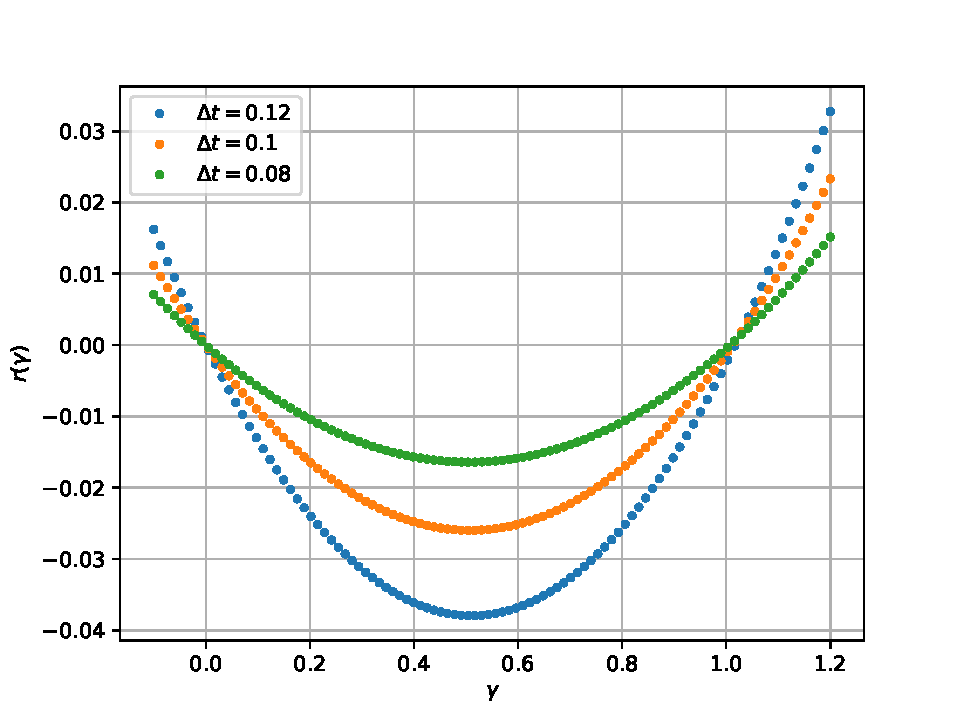
\includegraphics[width=0.50\textwidth]{figs/P1_r_of_gamma.pdf}}\hfill
        \subfloat[\(\left|r(\gamma = 1)\right|\) for some RK methods\label{Fig1b}] {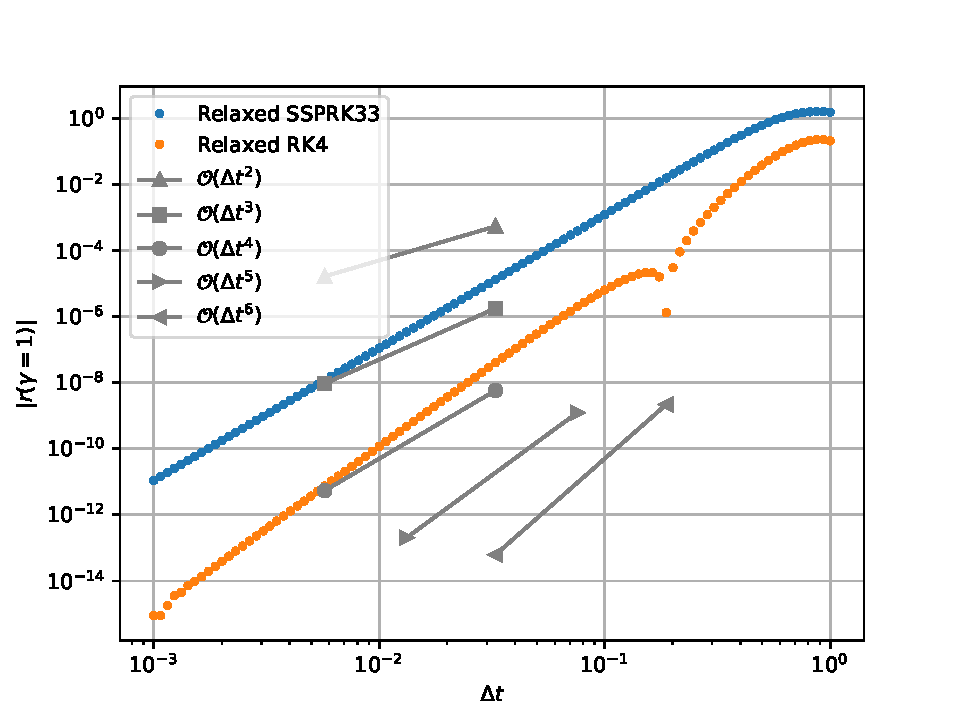
\includegraphics[width=0.50\textwidth]{figs/P1_r_at_1.pdf}}\hfill
        \caption{Numerical results for \(r\) at the first time step of problem 1.} \label{Fig1}
    \end{figure}
\end{frame}

\begin{frame}{Problem 1, cont.}
    \begin{figure}[H]
        \centering
        \subfloat[Classic methods\label{Fig2a}]{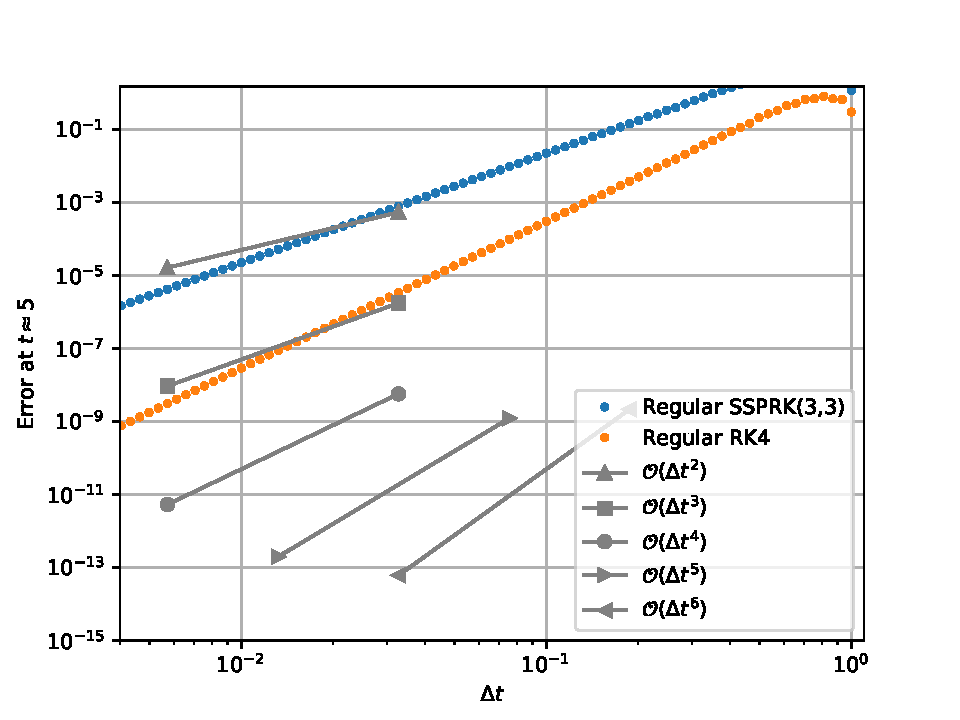
\includegraphics[width=0.33\textwidth]{figs/P1_Regular_RK4.pdf}}\hfill
        \subfloat[RRK Methods\label{Fig2b}] {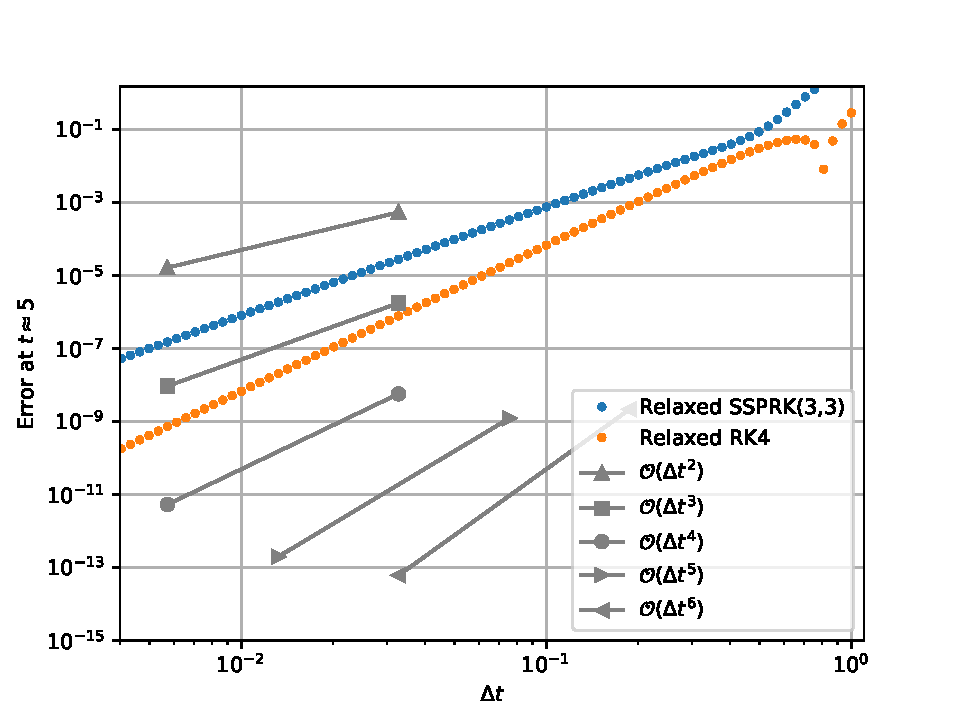
\includegraphics[width=0.33\textwidth]{figs/P1_Relaxed_RK4.pdf}}\hfill
        \subfloat[IDT methods\label{Fig2c}] {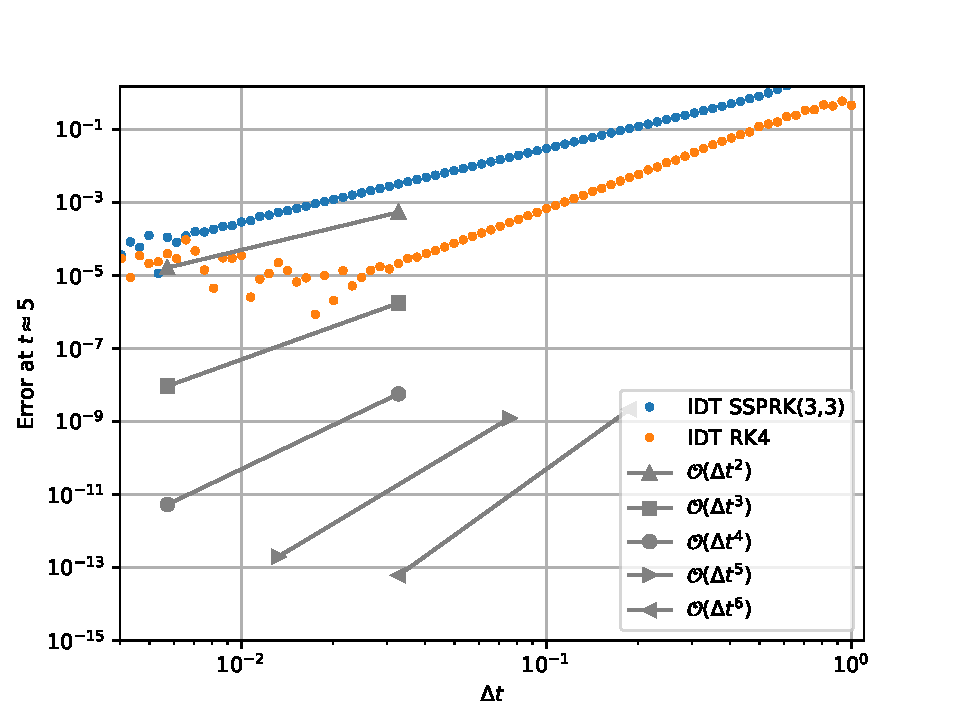
\includegraphics[width=0.33\textwidth]{figs/P1_IDT_RK4.pdf}}\hfill
        \caption{Convergence study for problem 1.} \label{Fig2}
    \end{figure}
\end{frame}

\begin{frame}{Problem 2 - Dissipated exponential entropy}
    Consider the ODE
    \[\frac{\text{d}}{\text{d}t} u(t) = -\expalt(u(t)), \qquad u^0 = 0.5,\]
    with the exponential entropy
    \[\eta(u) = \expalt(u), \qquad \eta'(u) = \expalt(u),\]
    and analytical solution
    \[u(t) = -\log(\exp{-1/2}+t).\]
\end{frame}

\begin{frame}{Problem 2, cont.}
    \begin{figure}[H]
        \centering
        \subfloat[\(r(\gamma)\) for SSPRK(3,3)\label{Fig3a}]{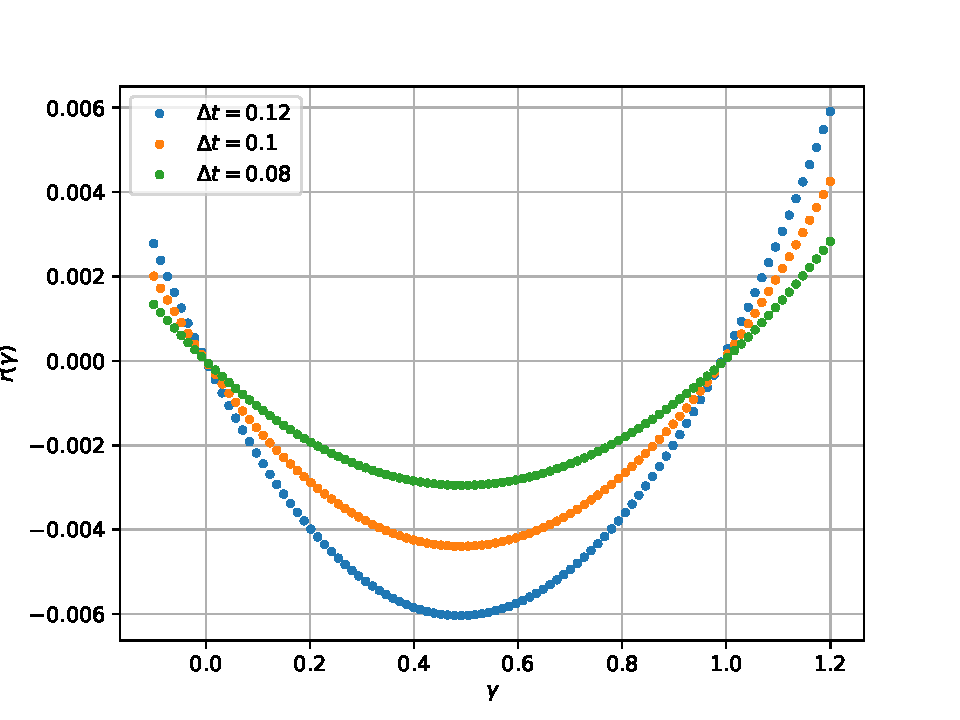
\includegraphics[width=0.48\textwidth]{figs/P2_r_of_gamma.pdf}}\hfill
        \subfloat[\(\left|r(\gamma = 1)\right|\) for some RK methods\label{Fig3b}] {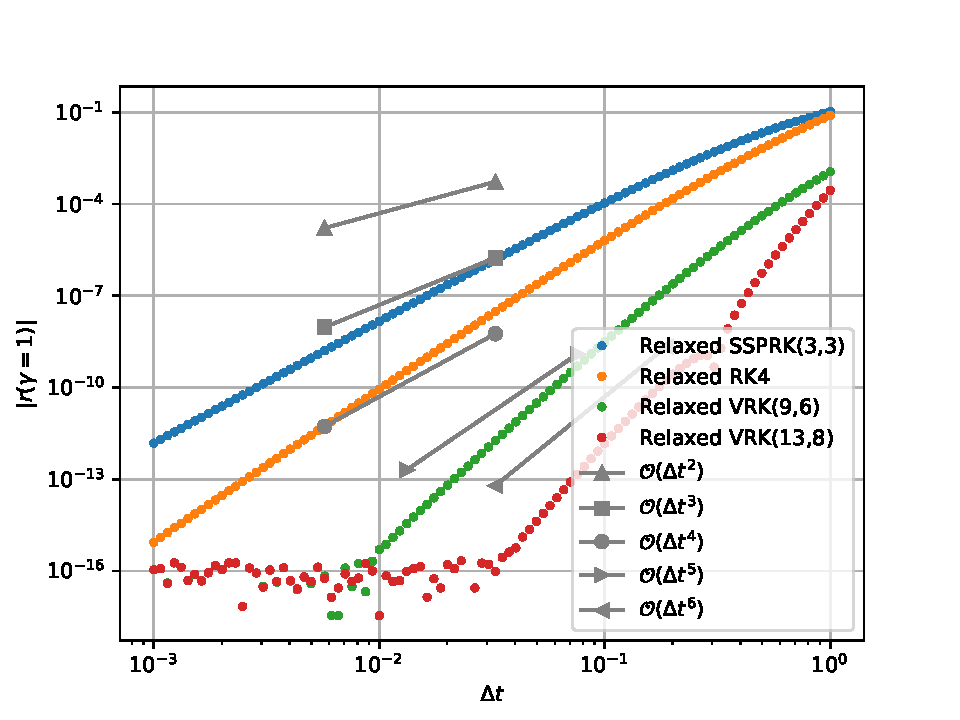
\includegraphics[width=0.48\textwidth]{figs/P2_r_at_1.pdf}}\hfill
        \caption{Numerical results for \(r\) at the first time step of problem 2.} \label{Fig3}
    \end{figure}
\end{frame}

\begin{frame}{Problem 2, cont.}
    \begin{figure}[H]
        \centering
        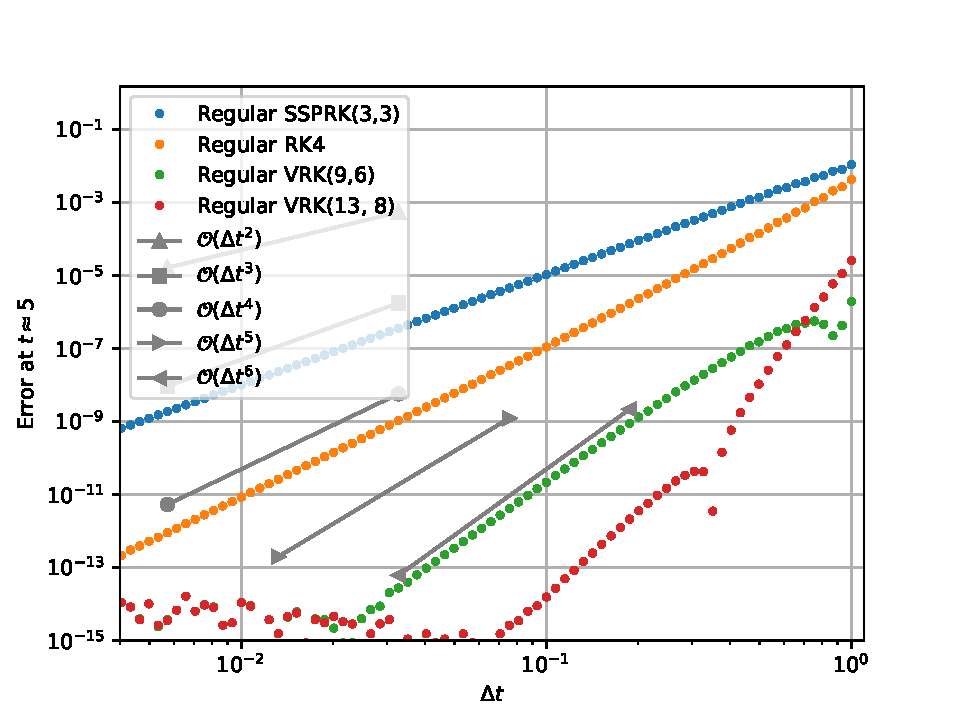
\includegraphics[width=0.75\textwidth]{figs/P2_Regular_RK4.pdf}
        \caption{Convergence study for problem 2, classic methods.}
        \label{Fig4a}
    \end{figure}
\end{frame}

\begin{frame}{Problem 2, cont.}
    \begin{figure}[H]
        \centering
        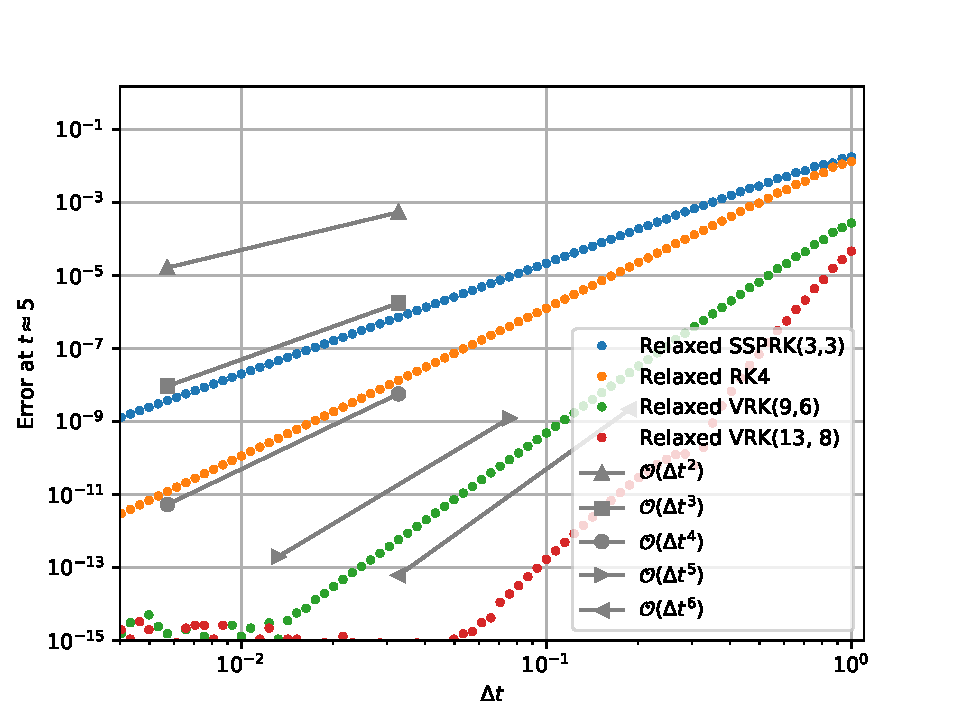
\includegraphics[width=0.75\textwidth]{figs/P2_Relaxed_RK4.pdf}
        \caption{Convergence study for problem 2, relaxed methods.}
        \label{Fig4b}
    \end{figure}
\end{frame}

\begin{frame}{Problem 2, cont.}
    \begin{figure}[H]
        \centering
        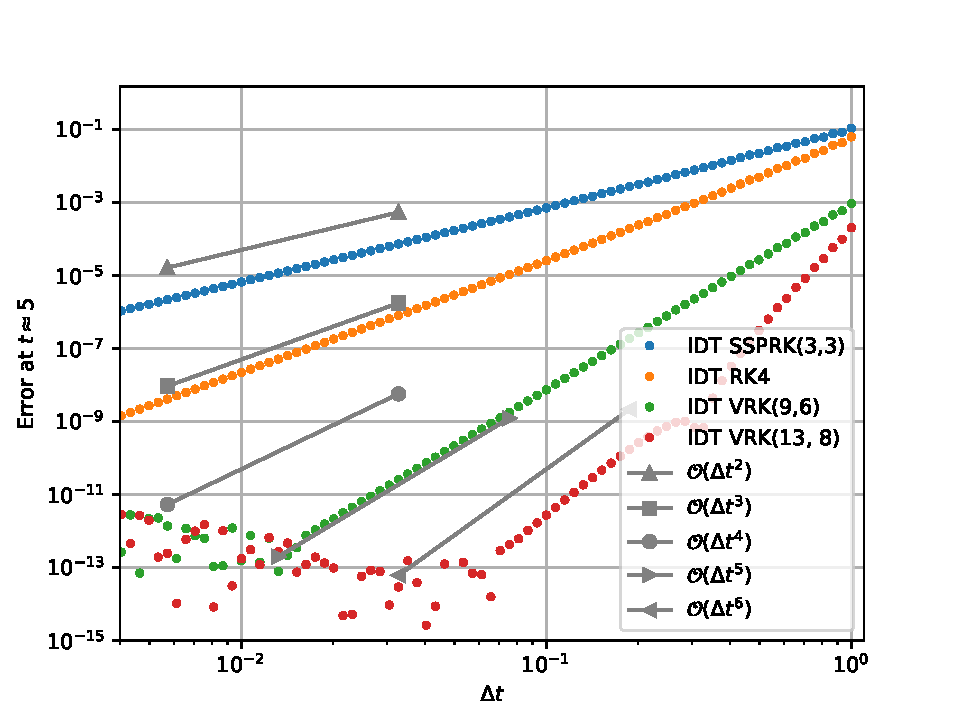
\includegraphics[width=0.75\textwidth]{figs/P2_IDT_RK4.pdf}
        \caption{Convergence study for problem 2, IDT methods.}
        \label{Fig4c}
    \end{figure}
\end{frame}

\section{Conclusion}
\begin{frame}{Conclusion}
    \begin{itemize}
        \item Simple
        \item Cheap
        \item Physically correct
        \item Requires \(\eta\)
    \end{itemize}
\end{frame}
\end{document}